\documentclass[a5paper]{article}
\usepackage[a5paper, top=8mm, bottom=8mm, left=8mm, right=8mm]{geometry}

\usepackage{polyglossia}
\setdefaultlanguage[babelshorthands=true]{russian}

\usepackage{fontspec}
\setmainfont{FreeSerif}
\newfontfamily{\russianfonttt}[Scale=0.7]{DejaVuSansMono}

\usepackage[font=scriptsize]{caption}

\usepackage{amsmath}
\usepackage{amssymb,amsfonts,textcomp}
\usepackage{color}
\usepackage{array}
\usepackage{hhline}
\usepackage{cite}

\usepackage[hang,multiple]{footmisc}
\renewcommand{\footnotelayout}{\raggedright}

\PassOptionsToPackage{hyphens}{url}\usepackage[xetex,linktocpage=true,plainpages=false,pdfpagelabels=false]{hyperref}
\hypersetup{colorlinks=true, linkcolor=blue, citecolor=blue, filecolor=blue, urlcolor=blue, pdftitle=1, pdfauthor=, pdfsubject=, pdfkeywords=}

\usepackage{tabu}

\usepackage{graphicx}
\usepackage{indentfirst}
\usepackage{multirow}
\usepackage{subfig}
\usepackage{footnote}
\usepackage{minted}

\sloppy
\pagestyle{plain}

\title{Примитивы синхронизации}
\author{Юрий Литвинов\\\small{yurii.litvinov@gmail.com}}

\date{08.09.2020}

\begin{document}

\maketitle
\thispagestyle{empty}

\section{Синхронизация}

Прошлая лекция заканчивалась весьма депрессивным примером \textit{гонки} --- ситуации, когда результат работы программы зависел от случайного порядка переключения потоков планировщиком. Гонки чаще всего возникают при попытке выполнить операции с переменными, разделяемыми между потоками (если более точно, операции с общими областями памяти). При этом читать значение переменной одновременно можно безопасно, а вот запись с чтением, и тем более запись с записью, сочетаются весьма плохо. Потокам надо как-то договориться, кто в какой последовательности что делает, и, собственно, этим и занимаются механизмы синхронизации.

Лучший способ синхронизации потоков --- это сделать так, чтобы она была вообще не нужна. Бывают (и на удивление часто) такие задачи, которые элементарно распараллеливаются и решаются разными потоками от начала до конца, возможно, синхронизируясь только в конце для получения итогового ответа. Пример такой задачи (про суммирование массива) был в прошлой лекции, ещё один такой пример --- умножение матриц.

Если синхронизация всё-таки нужна, она требует поддержки либо со стороны операционной системы, либо со стороны самого процессора. Собственно, поэтому примитивы синхронизации делятся на:

\begin{itemize}
    \item User-mode-примитивы --- атомарные операции, реализующиеся на процессоре и не требующие участия планировщика. Называются User-mode, потому что операционная система о них ничего не знает и никак в процессе не участвует. Пример такой операции --- процессорная инструкция инкремента, доступная из .NET через класс Interlocked, метод \mintinline{csharp}|Interlocked.Increment()|. Она просто увеличивает значение переданной переменной на 1 атомарно, то есть операция либо проходит полностью, либо не проходит вообще.
    \item Kernel-mode-примитивы --- примитивы, управляющие тем, как поток обрабатывается планировщиком. Поскольку это требует участия операционной системы, и, соответственно, переключения в режим ядра ОС, Kernel-mode-синхронизация работает гораздо медленнее user-mode и до 1000 раз медленнее ``без синхронизации вообще''. Зато с её помощью можно делать то, что user-mode-синхронизация в принципе не может --- например, ожидание без загрузки процессора (надо понимать, что у процессора нет инструкции ``подождать'', поэтому без планировщика он вынужден работать как проклятый, исполняя программу, даже если это бесконечный цикл в духе ``событие уже произошло? а сейчас? а сейчас?''). Ещё Kernel-mode-синхронизация позволяет синхронизировать даже разные процессы.
\end{itemize}

\section{Атомарные операции}

Сегодня мы очень кратко затронем работу с user-mode-примитивами, поскольку, с одной стороны, это потребуется для понимания концепций, важных в любых многопоточных программах, но с другой стороны, подробно рассматривать мы их не будем, потому что это неизбежно приведёт к теме lock-free-программирования, которое считается чёрной магией даже среди опытных параллельных программистов\footnote{Во всех книжках, что я про это читал, пишут в самом начале, что если вам понадобилось lock-free, подумайте ещё раз. И не пользуйтесь им никогда --- а теперь, когда вы осознали эту мысль, мы вам подробно про него расскажем}. Тем не менее, выпускники матмеха должны и чёрной магией владеть, так что мы ещё вернёмся к этой теме в следующем семестре.

Итак, атомарные операции, которые не могут быть прерваны посередине и всегда либо выполняются целиком, либо не выполняются вообще, это прежде всего операции чтения и записи типов, которые целиком помещаются в машинное слово. В .NET это конкретно Boolean, Char, (S)Byte, (U)Int16, (U)Int32, (U)IntPtr, Single, все ссылочные типы (потому что ссылочные типы --- это на самом деле указатели). Это не значит, что чтение и запись в переменные этих типов совершенно безопасны и можно делать это из нескольких потоков сразу, это всего лишь значит, что вы не прострелите себе ногу ещё одним интересным образом. Положим, у нас есть значение типа Int64 изначально там было 0000. Один поток пишет туда значение 1111, другой в это же время читает. При удачном тайминге (и если предположить для простоты, что размер машинного слова у нас <<две цифры>>), читающий поток может получить значение 0011, тогда как на самом деле переменная никогда в своей жизни таким значением не обладала. Атомарность чтения и записи означает лишь, что вот такой ерунды не случится.

\section{Модель памяти}

Ещё одна очень важная вещь, связанная с атомарностью операций, это \textit{модель памяти}: логическая модель того, как ведёт себя память, кеш и ядра процессора с точки зрения прикладного многопоточного программиста. Модель памяти сильно зависит от аппаратной архитектуры процессора, потому что чем меньше ограничений она накладывает, тем быстрее может работать процессор, но тем труднее его программировать. Хорошая новость в том, что самые распространённые архитектуры --- x86 и AMD64 --- придерживаются единой модели памяти, достаточно строгой, то есть \textbf{почти} ничего плохого не делают. Тем не менее, привыкать к хорошему нельзя --- другие архитектуры, например, Itanium (IA64), SPARC с удовольствием откусят вам руку, если вы не знаете, что делаете. Казалось бы, кому какое дело до SPARC, но именно эта архитектура выбрана основой XBox360 и PlayStation 3, например. Так что если вы вдруг захотите заняться серьёзным геймдевом, вас могут ждать сюрпризы.

Концептуально модель памяти описывает то, как ядра процессора пишут в память и как они переставляют инструкции на конвейере. Насчёт записи в память концептуально дела устроены как на картинке:

\begin{tabu} {X[1 c p] X[1 c p]}
    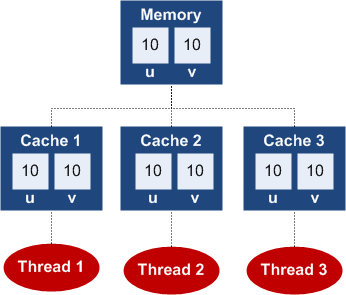
\includegraphics[width=0.35\textwidth]{volatile1.png} & 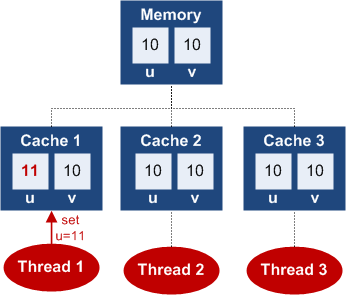
\includegraphics[width=0.35\textwidth]{volatile2.png} \\
    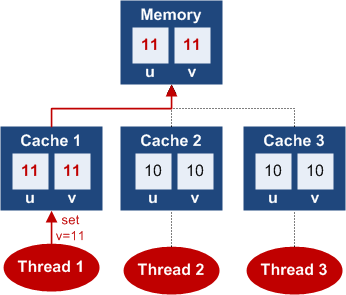
\includegraphics[width=0.35\textwidth]{volatile3.png} & 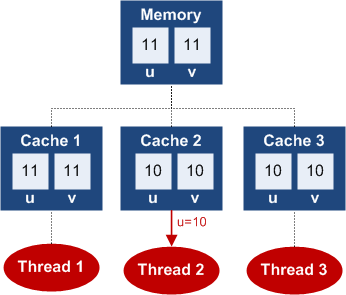
\includegraphics[width=0.35\textwidth]{volatile4.png} \\
\end{tabu}

Положим, каждый поток исполняется на своём ядре, и у них есть разделяемые переменные u и v. Изначально в них 10. Положим, первый поток пишет в u 11, сначала это значение попадает в кеш, и, вообще говоря, не обязано попасть в память. Довольно многие архитектуры не скидывают значение в память сразу, а ждут, пока значений накопится достаточно, чтобы записать их все одним запросом. Чтобы попросить ядро точно скинуть значения из кеша в память, нам потребуется специальная машинная инструкция volatile-записи, которая буквально и говорит ``запиши значение в кеш и тут же скинь кеш в память''. В нашем примере поток 1 выполняет volatile-запись значения v, сразу записывая 11 в кеш, и скидывая все значения из кеша в память. Обратите внимание, \textbf{все} значения из кеша, так что значение v, которое мирно лежало в кеше, тоже запишется. 

Теперь, положим, поток 2 хочет считать значение u из памяти. Он его читает, но читает из своего кеша, который ничего про изменения в памяти не знает, так что в качестве значения u придёт 10. Чтобы получить свежее значение, надо опять-таки воспользоваться машинной инструкцией volatile-чтения, которое имеет семантику ``обнови все имеющиеся значения в кеше и верни значение запрошенной переменной''.

На самом деле, как было сказано выше, модель памяти процессоров x86 и AMD64 умеет синхронизировать кеши, так что такие эффекты обычно не наблюдаются. ``Обычно'', потому что бывают буферы чтения-записи между кешем и регистром, они не синхронизируются. Тем не менее, прикладной программист может руководствоваться не особенностями конкретного процессора, а моделью памяти платформы. Конкретно модель памяти .NET чуть слабее, чем реализация x86: она декларирует, что все операции записи (даже обычные) исполняются как volatile, но операции чтения кеш не обновляют (то есть не volatile, даже несмотря на то, что процессор кеш обновит). Подробности см. в блоге Игоря Островского\footnote{Volatile keyword in C\# --- memory model explained, URL: \url{https://igoro.com/archive/volatile-keyword-in-c-memory-model-explained/} (дата обращения 03.09.2020)}, оттуда же без всякого согласия автора позаимствованы иллюстрации (для образовательных целей это, кажется, допустимо). Для тех, кто не боится лонгридов, очень рекомендую статью ``Memory Barriers: a Hardware View for Software Hackers''\footnote{McKenney P. E. Memory barriers: a hardware view for software hackers //Linux Technology Center, IBM Beaverton. – 2010, URL: \url{http://www.rdrop.com/users/paulmck/scalability/paper/whymb.2010.07.23a.pdf}}, там всё изложено во всех ужасных деталях.

Для тех, кто лонгриды не любит, есть простое, хотя и грубоватое правило --- все обращения к разделяемым переменным должны быть volatile. На некоторых архитектурах volatile-операции исполняются в десятки раз медленнее обычных (что не удивительно), так что более точное правило --- последняя операция записи и первая операция чтения, если у вас несколько записей подряд, или несколько чтений соответственно, должны быть volatile --- типа накидали в кеш значений, а потом скинули в память их все сразу. Если хотите ещё быстрее и лучше, читайте лонгрид.

\end{document}
